Questo capitolo verifica le ipotesi H2 e H3 e studia il comportamento di STERA quando i pesi si avvicinano al limite della memoria disponibile. Descriviamo prima i kernel che operano sulle coordinate, poi la banda di lettura del disco, il peso dei modelli, il confronto fra i due motori dello stesso STERA 30M, l'inferenza dei tre modelli del confronto linguistico e infine l'esecuzione con pesi che superano la memoria. Per leggere i risultati distinguiamo il tempo al primo token, che include l'elaborazione del prompt, il decode, cioè la produzione dei token successivi, e il tempo totale della richiesta.

\section{Due kernel per RowMask23}

Le misure richiedono due operazioni che non esistono nelle librerie standard. Le abbiamo scritte come kernel Metal, eseguiti sulla GPU del chip M1 attraverso l'interfaccia C++ di MLX.

\subsection{Espansione delle coordinate}

Il primo kernel espande le coordinate di una matrice nella matrice densa corrispondente. Ogni thread della GPU calcola un elemento: dalla sua posizione $(r,c)$ ricava il blocco a cui appartiene, la posizione $(i,j)$ dentro il blocco e l'indice $s=i\oplus j$; legge quindi la diagonale, la base ed eventualmente la correzione dal vettore delle coordinate del blocco e scrive il risultato moltiplicato per la scala. Per sapere se una posizione ha una correzione, e quale, il kernel usa una piccola tabella precalcolata di $128\times128$ elementi, la stessa per tutti i blocchi. Il risultato è identico, bit per bit, a quello della ricostruzione di riferimento usata durante l'addestramento; il controllo è eseguito automaticamente su ogni matrice prima delle misure.

\subsection{Prodotto diretto sulle coordinate}

Il secondo kernel calcola $y=Wx$ senza mai costruire $W$, applicando la formula \eqref{eq:gemv} con la trasformata di Walsh--Hadamard. La GPU lancia un gruppo di $128$ thread per ogni blocco della matrice. Ogni gruppo esegue questi passi:
\begin{enumerate}
\item carica in memoria condivisa le $3.176$ coordinate del blocco e i $128$ elementi del segmento di ingresso;
\item esegue in parallelo le trasformate di Walsh--Hadamard della base e del segmento di ingresso, in sette stadi separati da barriere di sincronizzazione;
\item moltiplica le due trasformate elemento per elemento e applica la trasformata inversa;
\item aggiunge per ogni riga il contributo della diagonale e delle $23$ correzioni, leggendo gli elementi dell'ingresso agli indici $i\oplus\sigma(i,k)$;
\item scrive il risultato parziale del blocco.
\end{enumerate}
I risultati parziali dei blocchi che stanno sulla stessa riga della matrice vengono infine sommati. Nel nostro kernel la trasformata della base è ricalcolata a ogni chiamata invece di essere memorizzata: in questo modo in memoria restano soltanto le coordinate, senza alcuna tabella ausiliaria per blocco.

La correttezza del prodotto diretto è verificata confrontandolo con il prodotto ottenuto espandendo la matrice; sui prompt usati nelle misure, i motori compatto e denso producono la stessa sequenza di token.

\section{Impostazione dei benchmark sul modello addestrato}
\label{sec:sistemi-impostazione}

\paragraph{Hardware.} Tutte le misure di inferenza della tesi sono state effettuate su un MacBook Air con chip Apple M1, 16 GiB di memoria unificata e SSD interno. Si distinguono la dimensione dei pesi persistenti e la memoria fisica occupata dall'intero processo: non sono grandezze intercambiabili.

\paragraph{Unico checkpoint STERA.} Il modello linguistico allenato è soltanto \textbf{STERA 30M}, con \num{30346182} parametri compatti e \num{82721280} elementi nella rappresentazione densa equivalente. Per isolare l'effetto dei motori, viene confrontato il percorso MLX/Metal che utilizza direttamente le coordinate con quello che carica le matrici densi ricostruite dallo stesso insieme di pesi. Tutti i test con tale coppia eseguono la medesima funzione appresa, e la coincidenza dei token generati è stata controllata sui prompt misurati.

\paragraph{Riferimenti pubblici.} Per le prove applicative sono eseguiti esclusivamente TinyStories-8M e TinyStories-33M, con un runtime PyTorch/MPS ottimizzato. Le differenze tra runtime, librerie e checkpoint impediscono di attribuire un eventuale divario di latenza alla sola struttura delle matrici. Il confronto più controllato riguarda i due motori di STERA 30M.

\paragraph{Metriche.} Il primo token include l'elaborazione del prompt. Il \emph{decode} misura il ritmo di emissione dei token successivi, con modello e cache già inizializzati. Dove indicato, ogni statistica è una mediana su input o ripetizioni a caldo. Il caricamento dei pesi viene escluso dalle latenze di richiesta a caldo, mentre i test di streaming da SSD sono riportati separatamente.

\paragraph{Pesi oltre la RAM.} Le misure di lettura fisica usano volumi controllati e contatori del dispositivo. Un termine di lettura non coincide con una generazione end-to-end. Il prototipo STERA di scala maggiore descritto alla fine del capitolo non ha subito un training linguistico completo e non viene inserito nei confronti qualitativi.

\section{Misura verificata dell'I/O su SSD}
\label{sec:ssd-io-verificato}

Per discutere l'esecuzione fuori RAM occorre conoscere la banda di lettura effettiva del disco, misurata in modo che i byte provengano davvero dal supporto fisico e non dalla cache del sistema operativo. La misura usa un file temporaneo fisicamente allocato di 256~MiB, riempito con dati pseudocasuali e sincronizzato, letto in sequenza con \texttt{F\_NOCACHE}, buffer e offset allineati. I volumi equivalenti al payload compatto F10 e al payload denso sono stati riletti più volte, con richieste fino a 1~MiB e ordine alternato delle prove. Il contatore aggregato del dispositivo ha registrato oltre il 99\% del payload atteso: i dati sono quindi stati letti effettivamente dal supporto.

\begin{table}[htbp]
\centering
\small
\begin{tabular}{lrrr}
\toprule
Volume nominale & Byte letti (GB) & Mediana (s) & Banda (GB/s) \\
\midrule
Pesi compatti equivalenti F10 & 4,003 & 1,685 & 2,375 \\
Pesi densi equivalenti F10 & 18,597 & 7,821 & 2,378 \\
\bottomrule
\end{tabular}
\caption{Lettura sequenziale validata su SSD del Mac M1: tre repliche per volume, dati temporanei e controllo dei byte fisicamente letti. GB è decimale.}
\label{tab:ssd-io-validato}
\end{table}

Una politica che dovesse rileggere integralmente 18,597~GB per ciascun token avrebbe quindi un termine di sola lettura dell'ordine di $7{,}82$~s a quella banda; il reciproco, circa $0{,}128$ token/s, è un tetto imposto dal solo I/O \emph{per quella politica}. Il calcolo, la latenza, lo staging e l'eventuale residenza parziale possono modificarne il risultato reale. La pipeline a doppio buffer può sovrapporre trasferimento e calcolo, ma non eliminare il tempo necessario ai byte effettivamente letti.

Questo termine di lettura è un limite inferiore al costo di una generazione che debba trasferire i pesi dal disco a ogni token; l'esempio completo di generazione con caricamento progressivo degli strati è discusso nella Sezione~\ref{sec:qwen-f10-ssd}.

\section{Quanto modello entra in un dispositivo}

Un limite analitico aiuta a distinguere la capacità di memorizzazione dal throughput. Un budget ipotetico di 12~GB per i soli valori FP16 contiene 6 miliardi di scalari densi. Se ogni blocco $128\times128$ fosse rappresentato esclusivamente dalle sue \,\num{3176} coordinate RowMask23, il rapporto ideale fra elementi sarebbe $16384/3176\approx5{,}16$. Tale rapporto non può essere esteso automaticamente a un Transformer completo: embedding, guadagni, fattori a basso rango, cache KV, workspace e granularità dei blocchi consumano spazio. Il prototipo STERA di scala maggiore effettivamente contabilizzato, discussa nella Sezione~\ref{sec:qwen-f10-ssd}, fornisce un confronto a scala maggiore con un perimetro esplicito.

\section{Peso di STERA 30M e quantizzazione}
\label{sec:stera30m-quantizzazione}

Il risparmio è $1-B_{\mathrm{STERA}}/B_{\mathrm{rif}}$, dove $B$ indica i byte nel perimetro dichiarato. La Tabella~\ref{tab:stera30m-byte} e la Figura~\ref{fig:byte-pesi} esplicitano il riferimento di ogni confronto. I payload FP32 dei checkpoint includono embedding, posizioni, bias e normalizzazioni. MB indica milioni di byte.

\begin{table}[htbp]
\centering
\small
\begin{tabularx}{\linewidth}{Xrrr}
\toprule
Confronto & STERA (MB) & Riferimento (MB) & Riduzione \\
\midrule
Compatto FP32 vs TinyStories-33M FP32 & 121,385 & 274,056 & 55,71\% \\
Compatto FP32 vs propria espansione FP32 & 121,385 & 330,885 & 63,32\% \\
Coordinate INT8 vs compatto FP32 & 74,241 & 121,385 & 38,84\% \\
Coordinate INT8 vs TinyStories-33M FP32 & 74,241 & 274,056 & 72,91\% \\
Coordinate INT8 vs propria espansione FP32 & 74,241 & 330,885 & 77,56\% \\
Archivio lossless vs propria espansione FP32 & 102,353 & 330,885 & 69,07\% \\
\bottomrule
\end{tabularx}
\caption{Confronti di peso per STERA 30M. Le righe FP32 e INT8 riportano payload numerici. L'ultima riga confronta i byte dell'archivio con il payload espanso FP32.}
\label{tab:stera30m-byte}
\end{table}

\begin{figure}[htbp]
\centering
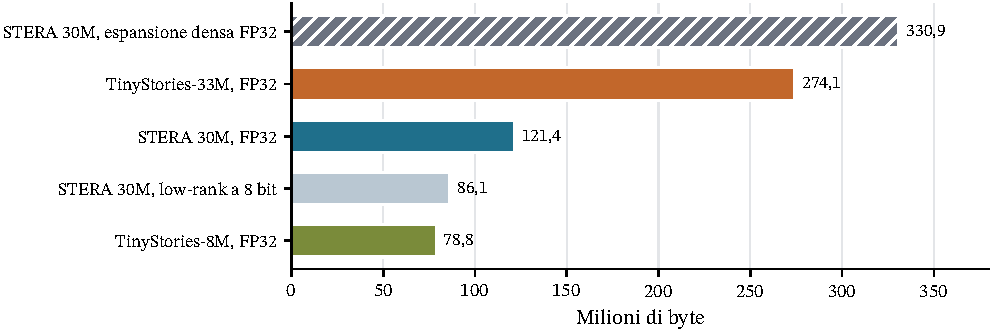
\includegraphics[width=.95\linewidth]{figure/risultati/byte_pesi_stera30m.pdf}
\caption{Byte occupati dai pesi di STERA 30M nelle diverse rappresentazioni, confrontati con i checkpoint TinyStories in FP32 e con l'espansione densa dello stesso modello.}
\label{fig:byte-pesi}
\end{figure}

Il $55{,}71\%$ rispetto a TinyStories-33M deriva già dal conteggio dei parametri a pari precisione. Una variante quantizza a INT8 soltanto le \num{15721200} coordinate RowMask23, con una scala simmetrica FP32 aggiuntiva per ciascuno dei \num{4950} blocchi. I fattori $U,V$, i guadagni, le scale apprese dei blocchi, le posizioni, le normalizzazioni e i bias rimangono FP32. Il payload misto è di \num{74240928} byte e supera il 70\% di riduzione rispetto a entrambi i riferimenti densi FP32 della tabella.

Il modello valutato e misurato nei benchmark di velocità è il compatto FP32. Il suo archivio lossless conserva esattamente i pesi e riduce il volume su disco del $69{,}07\%$ rispetto al payload denso equivalente. Per raggiungere il 70\% esatto con questo denominatore, l'archivio dovrebbe pesare al massimo \num{99265536} byte. Questi rapporti riguardano pesi e archivio. Il footprint di inferenza è misurato separatamente.

\section{Memoria durante l'addestramento}

Durante l'addestramento di STERA 30M le matrici vengono espanse temporaneamente per i prodotti con le attivazioni. I due momenti di Adam sono associati ai parametri allenabili della rappresentazione compatta. In FP32, assumendo quattro copie per peso, gradiente e momenti, il conto teorico è di circa 486 MB per STERA 30M. L'analogo conto per gli stessi valori espansi trattati come parametri indipendenti darebbe circa 1.324 MB. Attivazioni, matrici temporanee e workspace incidono separatamente sul picco di training.

\section{Confronto dei due motori dello stesso STERA 30M}
\label{sec:replica-stera-dense}

I due motori MLX/Metal eseguono gli stessi pesi, quelli del checkpoint finale di STERA 30M, sullo stesso Mac, a pesi residenti e precisione FP32. Il percorso compatto usa le coordinate RowMask23. Il percorso Dense carica l'espansione equivalente. Entrambi usano prefill a blocchi, SDPA in decode, batch 1 e cache KV di capacità 512. I sei input contano 256 token ciascuno e l'ordine dei motori viene alternato. La misura è ripetuta in cinque campagne consecutive, per un totale di 30 coppie di richieste a caldo; durante le campagne la media di carico del sistema era compresa fra 2,7 e 4,6. In ogni coppia coincidono tutti i 101 ID greedy sia alla prima richiesta sia a caldo, e gli ID sono gli stessi in tutte le campagne.

\begin{table}[htbp]
\centering
\begin{tabular}{lrrr}
\toprule
Motore & Primo token (ms) & Decode (tok/s) & Totale (s) \\
\midrule
STERA 30M Dense & 36,7 & 102,13 & 1,016 \\
STERA 30M compatto & 75,5 & 158,83 & 0,704 \\
\bottomrule
\end{tabular}
\caption{Mediane a caldo su 30 misure appaiate (sei input in cinque campagne). Il caricamento dei pesi è escluso.}
\label{tab:replica-stera-dense}
\end{table}

\begin{figure}[htbp]
\centering
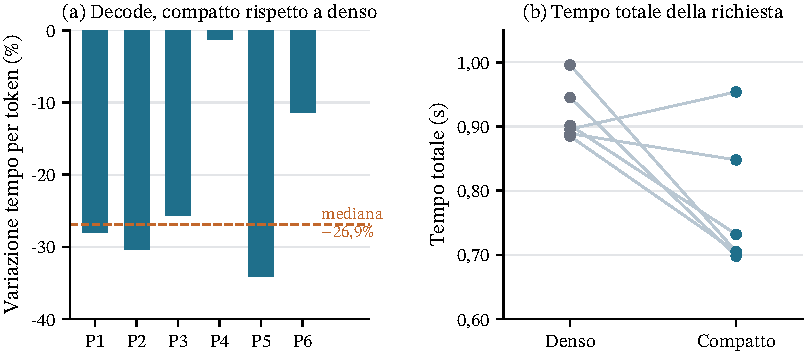
\includegraphics[width=\linewidth]{figure/risultati/decode_appaiato_stera30m.pdf}
\caption{Confronto appaiato fra il motore compatto e il motore denso sugli stessi pesi, per i sei input da 256 token; ogni valore è la mediana delle cinque campagne. (a) Variazione del tempo per token in decode. (b) Tempo totale della richiesta: ogni linea collega le due misure dello stesso input.}
\label{fig:decode-appaiato}
\end{figure}

La riduzione mediana appaiata del tempo per passo di decode è del $35{,}9\%$ (Figura~\ref{fig:decode-appaiato}), con riduzioni osservate da $31{,}3\%$ a $40{,}5\%$ sulle 30 coppie; le mediane delle singole campagne sono comprese fra $35{,}3\%$ e $36{,}4\%$. Il Dense emette prima il primo token in tutte le 30 coppie, mentre il compatto impiega meno tempo totale in tutte le 30. Il confronto dei soli payload FP32 vale 121,385 contro 330,885 MB. Questi valori descrivono i pesi, mentre cache, buffer e runtime contribuiscono alla memoria di esecuzione.

\section{Inferenza applicativa: STERA 30M e i due TinyStories}
\label{sec:tre-checkpoint-inferenza}

Riprendiamo i tre checkpoint del confronto di qualità della Sezione~\ref{sec:risultati-stera30m-tinystories}. La Tabella~\ref{tab:tre-checkpoint-ram} riporta separatamente il payload FP32 dei soli parametri e il footprint fisico di processo durante una richiesta. STERA 30M è rappresentato dal checkpoint finale. Lo stesso Mac M1 esegue ogni braccio su GPU, a pesi residenti, con batch 1, 256 token in ingresso e 100 passi dopo il primo token. I tempi sono le mediane di 15 richieste a caldo, tre input identici fra i modelli ripetuti nelle stesse cinque campagne del confronto precedente. Il picco è il massimo campionato ogni 10 ms durante la richiesta a caldo, in mediana sulle 15 misure. Include le allocazioni trattenute dal runtime.

\begin{table}[htbp]
\centering
\small
\begin{tabular}{lrrrr}
\toprule
Checkpoint & Pesi FP32 & Primo token & Decode & Picco RAM \\
 & (MB) & (ms) & (tok/s) & (MiB) \\
\midrule
TinyStories-8M & 78,810 & 21,8 & 176,55 & \num{1525.18} \\
STERA 30M & 121,385 & 121,3 & 160,03 & \num{412.89} \\
TinyStories-33M & 274,056 & 31,8 & 94,79 & \num{1493.07} \\
\bottomrule
\end{tabular}
\caption{Inferenza FP32 sul Mac M1. Il massimo di RAM si riferisce al footprint fisico di processo osservato durante la richiesta.}
\label{tab:tre-checkpoint-ram}
\end{table}

STERA usa il motore MLX/Metal sulle coordinate compatte. TinyStories usa GPT-Neo su PyTorch/MPS con adattatore SDPA e proiezione dell'ultimo token nel prefill. Per ognuno dei due TinyStories, i 101 ID prodotti coincidono con quelli dell'implementazione eager su tutti e tre gli input, in ogni campagna. I due TinyStories rispondono prima al primo token. In decode STERA 30M è più rapido del 33M e più lento dell'8M. Il totale mediano della richiesta è di $0{,}591$ s per l'8M, $0{,}745$ s per STERA 30M e $1{,}088$ s per il 33M: STERA 30M completa quindi la richiesta prima del 33M (68,5 milioni di parametri), mentre l'8M (19,7 milioni) resta più rapido. Il footprint include il costo del framework, e i risultati descrivono le implementazioni provate.

\paragraph{Budget di addestramento.} STERA 30M è addestrato su \num{1529514422} token bersaglio, escluso il riempimento. L'autore di TinyStories-33M \href{https://huggingface.co/roneneldan/TinyStories-33M/discussions/8}{dichiara circa 20 epoche}. Sedici campioni del file ufficiale, tokenizzati con il BPE pubblico, danno una stima di circa 475 milioni di token per passaggio e circa 9,5 miliardi su 20 passaggi. È un ordine di grandezza basato sul tokenizzatore disponibile; per TinyStories-8M il totale non è documentato. I riferimenti hanno quindi visto un numero di token sensibilmente maggiore di STERA 30M.

\section{Confronto finale di sistema: prototipo STERA non addestrato e Qwen3.5-9B}
\label{sec:qwen-f10-ssd}

\paragraph{Che cosa è il prototipo grande.} Per studiare il limite di memoria, è stata realizzata una configurazione \emph{STERA F10} di scala maggiore rispetto a STERA 30M. I suoi pesi compatti sono inizializzati deterministicamente a partire dal checkpoint finale di STERA 30M: \textbf{non è un secondo modello linguistico addestrato}. Esegue effettivamente il forward e il decode, ma le sue generazioni non dimostrano qualità narrativa, generalizzazione o prestazioni linguistiche di un ipotetico modello grande addestrato da zero.

\paragraph{Dimensione e soglia di RAM.} Il payload contabilizzato dal loader del prototipo compatto FP32 è 4,003~GB, ovvero 3,73~GiB. La rappresentazione densa equivalente richiederebbe una stima complessiva di 18,597~GB (17,32~GiB) di soli pesi, più della memoria fisica del Mac (Figura~\ref{fig:soglia-ram-f10}). La riduzione del payload rispetto alla stima densa è del $78{,}48\%$. La stima comprende il perimetro di parametri dichiarato nel report del loader; cache e workspace sono esclusi dai byte dei pesi.

\begin{figure}[htbp]
\centering
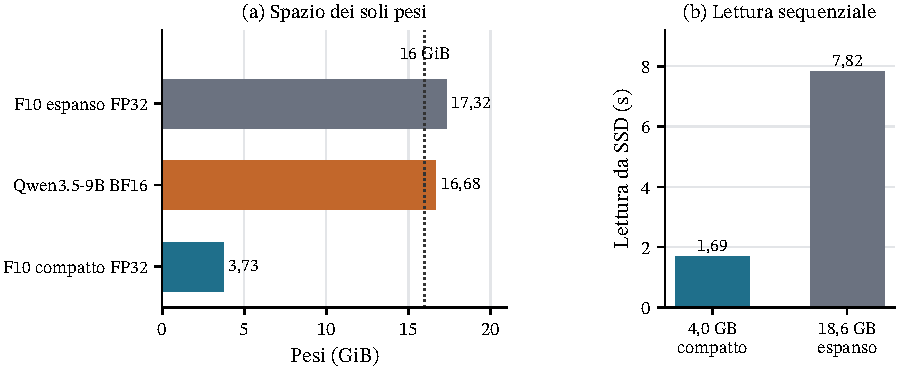
\includegraphics[width=\linewidth]{figure/risultati/soglia_ram_m1.pdf}
\caption{(a) Spazio occupato dai soli pesi del prototipo F10 in forma compatta ed espansa e di Qwen3.5-9B in BF16, rispetto ai 16~GiB di memoria del dispositivo. (b) Tempo mediano di lettura sequenziale dall'SSD dei due volumi del prototipo F10.}
\label{fig:soglia-ram-f10}
\end{figure}

\paragraph{Decode con pesi residenti.} In due prove del motore MLX/Metal, il prototipo STERA non addestrato produce 9,89 e 9,73 token/s con un prompt breve di tre token e cache predisposta per 128 posizioni. Non sono prove di generazione linguistica valutabile. Il corrispondente prototipo denso fuori RAM non è stato eseguito in un test end-to-end appaiato.

\paragraph{Qwen3.5-9B come esempio indipendente.} Per verificare una strategia reale di offload da SSD è stato eseguito il decoder di Qwen3.5-9B, con pesi BF16, runtime SWLP su PyTorch/MPS, batch uno e lettura degli strati da SSD. Embedding e testa restano in RAM, mentre i blocchi attraversano una finestra di caricamento e prefetch. Il modello pubblico è addestrato, ma il suo ruolo qui riguarda esclusivamente i costi di esecuzione su memoria limitata: non è una baseline della qualità narrativa di STERA 30M.

\begin{table}[htbp]
\centering
\small
\begin{tabular}{rrrrr}
\toprule
Input (token) & Primo token (s) & Decode (tok/s) & Picco processo (GiB) & Letture SSD (GB) \\
\midrule
256 & 12,06 & 0,153 & 7,63 & 57,15 \\
\num{4096} & 95,55 & 0,147 & 7,45 & 154,50 \\
\bottomrule
\end{tabular}
\caption{Qwen3.5-9B in BF16 con SWLP, una prova per condizione, quattro token generati, prefetch attivo. Il decode comprende i tre passi successivi al primo; letture e picco includono il caricamento.}
\label{tab:qwen-swlp}
\end{table}

Con 256 token di input, una prova separata disattiva il prefetch e riporta 0,126 token/s nel decode, contro 0,153 con prefetch; il risparmio temporale osservato è del $17{,}6\%$ sui tre passi successivi al primo. Sono singole prove e non forniscono un intervallo sulla variabilità di esecuzione.

\paragraph{Termine di I/O e contesto lungo.} La lettura sequenziale validata di 18,597~GB dallo stesso SSD richiede una mediana di 7,821~s: è il costo della sola lettura fisica a quella banda. Una politica che rilegga tutto il volume a ogni token avrebbe quindi un limite imposto dall'I/O dell'ordine di 0,128 token/s, ma caching, residenza parziale e sovrapposizione del calcolo cambiano il risultato del sistema reale. Una simulazione analitica a 32.768 token stima l'effetto della cache KV e della residenza parziale; non è un test linguistico a contesto lungo del prototipo non addestrato. La prova di decode su cache sintetica piena non verifica la coerenza del testo oltre il contesto di training di STERA 30M.

\paragraph{Lettura dei risultati.} I due casi illustrano regimi di memoria diversi: pesi compatti interamente residenti da un lato, trasferimento continuo degli strati dal disco dall'altro. Poiché modelli, precisioni e runtime differiscono, il rapporto fra i rispettivi token/s descrive i due regimi e non va letto come un confronto di velocità a parità di modello.

\section{Sintesi}

Sullo stesso STERA 30M, il motore che applica le proiezioni direttamente alle coordinate riduce del $35{,}9\%$ il tempo mediano per token in decode rispetto al motore con matrici dense equivalenti, producendo gli stessi token; il motore denso resta più rapido nel primo token. I pesi compatti occupano 121,385~MB in FP32, il $63{,}32\%$ in meno della propria espansione densa, e 74,241~MB con le sole coordinate in INT8. A scala maggiore, la rappresentazione compatta del prototipo F10 resta interamente in memoria su un dispositivo da 16~GiB, mentre la sua espansione densa la supererebbe e richiederebbe il trasferimento dei pesi dal disco, con un costo di lettura misurato di circa 7,8~s per passaggio completo.
